%% Manuscript for Computers in Biology and Medicine (Elsevier)
%% Format: Elsevier CAS double-column class (cas-dc), converted from IEEEtran
%% Needs in the same folder (from the Elsevier CAS bundle): cas-dc.cls, cas-common.sty,
%%   model1-num-names.bst, plus your ref.bib and the figure PNGs.
%% Compile: pdflatex -> bibtex -> pdflatex -> pdflatex
\documentclass[a4paper,fleqn]{cas-dc}

\usepackage[numbers]{natbib}
\usepackage{amsmath,amssymb}
\usepackage{placeins}
\usepackage{xcolor}
\usepackage{subfig}
\usepackage{url}
\usepackage{float}
% \usepackage{capt-of}


\renewcommand{\topfraction}{0.9}
\renewcommand{\bottomfraction}{0.8}
\renewcommand{\textfraction}{0.1}
\renewcommand{\floatpagefraction}{0.7}
\renewcommand{\dbltopfraction}{0.9}
\renewcommand{\dblfloatpagefraction}{0.7}
\setcounter{topnumber}{3}
\setcounter{dbltopnumber}{3}
\setcounter{totalnumber}{5}
\newcommand{\leadfig}[3]{\subfloat[#1]{\includegraphics[width=0.24\textwidth,height=#3]{#2}}}


\begin{document}
\let\WriteBookmarks\relax
\shorttitle{Explainable Multi-Label ECG Classification}
\shortauthors{D. Fiuji et~al.}

\title [mode = title]{An Explainable Deep Learning Method for Multi-Label Cardiac Abnormality Classification From 12-Lead Electrocardiogram Signals}

\author[1]{Donya Fiuji}

\author[1]{Foad Ghaderi}[]
\cormark[1]
\ead{fghaderi@modares.ac.ir}

\author[1]{Behzad Akbari}

\affiliation[1]{organization={Human-Computer Interaction Lab., Faculty of Electrical and Computer Engineering, Tarbiat Modares University},
                city={Tehran},
                country={Iran}}

  
\cortext[cor1]{Foad Ghaderi}

\begin{abstract}
Since automatic analysis of electrocardiograms can play an important role in preventing cardiac diseases, numerous machine learning approaches have been developed for medical applications in recent decades. In clinical practice, a single ECG recording may simultaneously exhibit multiple cardiac abnormalities, making multi-label classification essential for realistic and reliable diagnosis. Moreover, when it comes to medical diagnosis and human life, model predictions must be trustworthy, particularly in the case of neural networks. In this study, we propose an explainable machine learning model for the multi-label classification of 12-lead ECG recordings from the PTB-XL dataset. The proposed approach employs a convolutional neural network (CNN) optimized to capture discriminative ECG features of the signal, combined with the Grad-CAM explainability technique, which backpropagates gradients and uses them to weight the corresponding feature maps, thereby producing heatmaps that highlight the input regions most influential to the model's decision. Experimental results on the PTB-XL dataset show that the proposed method achieves 88\% classification accuracy, a micro-average area under the curve (AUC) of 94\%, and an F1-score of 74.6\%. The study further examines the strengths and limitations of the proposed approach in comparison with recent multi-label and explainable ECG classification methods, along with directions for future work.
\end{abstract}

%% Highlights are NOT in the IEEE version; Elsevier asks for them at submission (upload as a separate file or uncomment):
%% \begin{highlights}
%% \item Multi-label classification of 12-lead ECGs with XResNet1D101 on PTB-XL
%% \item Class-wise F1-optimized thresholds improve multi-label decisions
%% \item Grad-CAM adapted to 1D ECG with channel-averaging alignment
%% \item Heatmaps localize QRS and P-wave regions driving each prediction
%% \end{highlights}

\begin{keywords}
Electrocardiogram \sep Explainable AI \sep Multi-label Classification \sep Grad-CAM \sep PTB-XL
\end{keywords}

\maketitle

\section{Introduction}
\label{sec:intro}
Cardiovascular diseases (CVDs) are the foremost cause of mortality worldwide, claiming approximately 17.9 million lives annually and accounting for 32\% of all global fatalities \cite{who}. Detecting cardiovascular disease at an early stage is crucial for initiating treatment with counselling and medications. CVDs comprise a variety of disorders affecting the heart and blood vessels, such as coronary heart disease, cerebrovascular disease, and rheumatic heart disease. Over 80\% of CVD deaths result from heart attacks and strokes, with a third of these occurring prematurely in individuals under the age of 70, according to the World Health Organization \cite{who}. The rising number of fatalities due to cardiovascular disease underscores the need for early diagnosis and the development of automated tools to identify major events through electrocardiogram (ECG) records. With the growing popularity and application of machine learning models in recent decades, significant efforts have been made to create high-performance decision systems via ECG analysis. Arrhythmias refer to abnormal heart rhythms caused by alterations in the heart's usual electrical impulse sequence and disturbances in its electrical conduction pathways. These can appear in any heart chamber, though ventricular arrhythmias are notably dangerous \cite{label2}. The ECG is essential for identifying such abnormalities, as it records the heart's electrical signals. Nonetheless, ECG signals have a low amplitude and low frequency range (0.5--150 Hz), making them prone to various noise types, such as power-line interference, electrode noise, motion artifacts, muscle contraction noise, baseline drift, and electrosurgical noise. Effective noise reduction is vital for precise ECG analysis. Multiple methods have been employed for denoising, including band-pass filtering \cite{shang2018removal}, wavelet denoising \cite{rodenas2018efficient}, adaptive filtering, empirical mode decomposition (EMD) \cite{dai2021denoising, xin2014ecg}, principal component analysis (PCA) \cite{romero2010pca}, independent component analysis (ICA) \cite{he2006application}, and median filtering \cite{xin2014ecg}. Enhancing the signal quality through these methods allows for a more accurate examination of individual ECG beats, providing critical insights into cardiac health. After successful denoising, various features can be extracted and classified based on clinical relevance and representation, aiding precise diagnosis and analysis. Although ECG analysis has greatly benefited from machine learning, clinical adoption of deep models is nonetheless hindered by their lack of interpretability. To address this gap, we propose an explainable artificial intelligence (XAI) approach using a convolutional neural network (CNN) for multi-label classification of 12-lead ECG signals, combined with Grad-CAM visualizations. In this approach, first the signals are analyzed to achieve reliable detection given the multi-label nature of the data, and then heatmaps are generated to assist in visualizing the results. The main contributions of this work can be categorized into:
\begin{itemize}
    \item Using a 1D residual CNN architecture (XResNet1D101) optimized for simultaneous detection of multiple cardiac abnormalities.
    \item A class-wise threshold tuning strategy that improves multi-label detection performance under imbalanced data.
    \item Adaptation of the Grad-CAM algorithm to 1D ECG signals, enabling temporal localization of clinically relevant waveform regions.
    \item Comprehensive evaluation and interpretation of model decisions, fostering transparency for real-world clinical deployment.
\end{itemize}
The remainder of this paper is organized as follows: Section~\ref{sec:related} reviews related work on ECG preprocessing, classification, and interpretability. Section~\ref{sec:methods} describes the proposed methodology, including the model architecture, multi-label threshold optimization, and Grad-CAM explainability. Experimental setup and results are presented in Section~\ref{sec:results}, followed by a discussion of findings and future directions in Section~\ref{sec:conclusion}.

%% ------------------------------------------------------------------
\section{Related Work}
\label{sec:related}
Electrocardiograms are a cornerstone in diagnosing cardiovascular diseases. Over the past two decades, extensive research has explored the use of signal processing, machine learning (ML), and deep learning (DL) methods for ECG noise suppression and classification. This section summarizes key prior studies focused on ECG preprocessing, classification, and approaches to model interpretability.

\subsection{Signal Preprocessing Techniques}
ECG signals are susceptible to various types of noise, such as baseline drift, power-line interference (PLI), muscle artifacts, and motion-induced distortions. Effective denoising enhances feature extraction and classification accuracy. Shea et al.~\cite{shea2024baseline} proposed the Derived Peak (DP) encoding method, a non-parametric approach to peak generation based on zero-crossings in first and second derivatives of the ECG. Their model, based on 1D-ResNet-18, maintained robust performance under signal perturbations, achieving an AUC of 88\%. Bellfield et al.~\cite{bellfield2024impact} studied the impact of input data format on ECG classification. Their results showed that for 10-second ECG windows, signal-based formats yielded the best performance, whereas for shorter 2.5-second signals, image-based formats were more effective. Despite significant advancements in ECG data analysis, achieving high accuracy and computational efficiency remains challenging. In addition, issues such as data imbalance and the need for models with strong generalization capabilities, as well as ensuring patient privacy, continue to pose major obstacles. To address challenges like generalization and data imbalance, Safdar et al.~\cite{safdar2023novel} introduced a novel augmentation technique using segment-wise rearrangement of ECG signals. A lightweight 4-layer CNN trained on the augmented signals achieved competitive accuracy with minimal computational cost. Bui et al.~\cite{bui2021comparison} examined Finite Impulse Response (FIR) and Infinite Impulse Response (IIR) filters at various sampling rates, optimizing the signal-to-noise ratio (SNR) and ensuring alignment between signal and system frequency. Ivanov et al.~\cite{ivanov2022convolutional} proposed a convolutional autoencoder (CAE) for removing PLI noise. The model was evaluated using root mean square error (RMSE) and percent root mean square difference (PRD) metrics, showing strong generalization to non-stationary interference.

\subsection{Deep Learning Techniques}
A wide range of deep learning models have been proposed to classify ECG signals. These models vary in complexity, input formats, and learning paradigms. While various datasets have been utilized historically, the literature reviewed in this section focuses specifically on studies employing the PTB-XL dataset. This narrow focus is necessitated by the requirement for a consistent benchmark; since our proposed method addresses multi-label classification in standard 12-lead ECGs, direct comparison with works using the same data and annotation standards is essential for a valid performance evaluation. Recent research on PTB-XL has explored diverse architectures and learning paradigms. Smigiel et al.~\cite{smigiel2021ecg} evaluated three architectures: a one-dimensional convolutional neural network (1D-CNN) on time series, SincNet, and a CNN with entropy-based features. Feyisa et al.~\cite{feyisa2022lightweight} proposed a multi-receptive field CNN (MRF-CNN) with varying kernel sizes. It has been structured in a way that allows different semantic contexts within the signals to be considered, thereby improving classification accuracy. Zhu et al.~\cite{zhu2022cnn} introduced CNN-FWS, integrating recursive feature elimination based on feature weights (FW-RFE) to improve input relevance. Pa{\l}czy{\'n}ski et al.~\cite{krzysztof2022study} used few-shot learning (FSL) with proximity-based classification. R-peak detection was also used for QRS segmentation. Smigiel et al.~\cite{smigiel2021deep} later integrated k-means clustering and entropy-based features for QRS extraction. Best results were obtained when combining raw signals, QRS features, and entropy measures, ensuring that the neural network benefits from the most relevant parts of the signal for learning. Yang et al.~\cite{yang2024fusion} also presented a ResNet-GRU hybrid with simplified self-attention for ECG classification across multiple diagnostic classes. Chorney et al.~\cite{chorney2024towards} proposed a federated learning model, using autoencoders for dimension alignment while preserving privacy. Chen et al.~\cite{chen2024improving} proposed a method that integrates demographic information into ECG classification by encoding metadata as RGB color channels. This information was combined with ECG signal inputs to enhance the model's contextual understanding. Saglietto et al.~\cite{saglietto2024convolutional} showed that a single-lead CNN could be used for ECG abnormality classification. Ramirez et al.~\cite{ramirez2024explainable} used Vectorcardiogram (VCG) and reconstructed ECG with inverse Dower transform for myocardial infarction detection. More recent studies have increasingly addressed the spatial relationships among ECG leads and the temporal dependencies within ECG signals, introducing architectures that explicitly model these complementary characteristics. Yang et al.~\cite{yang2025lead} investigated the spatial interdependence among ECG leads through a five-lead grouping strategy and proposed the L5G-Net architecture. Concurrently, hybrid temporal models combining 1D-CNN with gated recurrent units (GRUs) and channel attention have demonstrated high accuracies in temporal and heartbeat-level arrhythmia detection~\cite{sundaramoorthy2026explainable}. Table~\ref{table:literature_review} presents an overall summary of the previous works.

\begin{table*}[!t]
\centering
\caption{Summary of Prior Works on ECG Classification}
\label{table:literature_review}
\resizebox{\textwidth}{!}{%
\begin{tabular}{|l|c|c|c|c|c|}
\hline
\textbf{Study} & \textbf{Signal Format} & \textbf{Model} & \textbf{Labels} & \textbf{AUC/Acc} & \textbf{XAI} \\ \hline
Smigiel et al.~\cite{smigiel2021ecg} & Raw + Features & CNN/SincNet & 2,5,20 & 0.89/0.76/0.69 & No \\ \hline
Feyisa et al.~\cite{feyisa2022lightweight} & Raw & MRF-CNN & 5+ & 0.89 & No \\ \hline
Zhu et al.~\cite{zhu2022cnn} & Raw & CNN-FWS & 2 & 0.902 F1 & No \\ \hline
Pa{\l}czy{\'n}ski et al.~\cite{krzysztof2022study} & QRS Segments & FSL-CNN & 2,5,20 & +2--10\% over baseline & No \\ \hline
Smigiel et al.~\cite{smigiel2021deep} & Raw + QRS & DNN & 2,5,20 & 0.763 & No \\ \hline
Yang et al.~\cite{yang2024fusion} & Raw & ResNet+GRU & 5,23,44 & 0.88 Acc & No \\ \hline
Chorney et al.~\cite{chorney2024towards} & Raw & Federated Autoencoder & 5 & 0.73 Acc & No \\ \hline
Chen et al.~\cite{chen2024improving} & RGB+Raw & CNN & 2,5,15 & +1--6\% AUC & No \\ \hline
Saglietto et al.~\cite{saglietto2024convolutional} & Single-lead & CNN & 15 & 0.932 AUC & No \\ \hline
Ramirez et al.~\cite{ramirez2024explainable} & VCG + Rebuilt ECG & CNN & 2 & 0.895 Acc & Yes \\ \hline
Yang et al.~\cite{yang2025lead} & Raw 12-lead & L5G-Net (5-Group CNN) & 5, 24, 71 classes & 0.9357 AUC & No \\ \hline
Sundaramoorthy et al.~\cite{sundaramoorthy2026explainable} & Segmented 1D & 1D-CNN + GRU + Attn & MIT-BIH, INCART & 99.6\% Acc & Yes \\
\hline
\end{tabular}}
\end{table*}
\FloatBarrier

%% ------------------------------------------------------------------
\section{Materials and Methods}
\label{sec:methods}
The proposed study addresses the critical need for both accurate classification and interpretability in automated electrocardiogram analysis. Given the low amplitude and short duration of ECG signals, clinical interpretation is often subject to variability and error. Moreover, ECG recordings are frequently contaminated by various sources of noise, including muscle artifacts, power-line interference, baseline wandering, and motion artifacts, which can obscure clinically relevant patterns and adversely affect classification performance. Among these, baseline wandering appears as a low-frequency fluctuation that gradually shifts the ECG signal from its original baseline, making accurate waveform analysis more challenging (Fig.~\ref{fig:ecg_noise_examples}). These challenges underscore the importance of applying robust preprocessing and deep learning techniques capable of learning subtle patterns in ECG waveforms. In this work, we present a deep learning framework for multi-label classification of ECG signals, which includes multiple concurrent diagnostic labels per sample. This setting reflects real-world scenarios where patients often present with overlapping cardiac conditions. Our model is based on the XResNet1D101 architecture and is trained using a sliding-window augmentation strategy. To mitigate the effects of noise, the signals undergo a two-stage filtering process consisting of a high-pass filter for baseline wander removal and a moving average filter for smoothing, followed by standardization. Data splits follow the predefined folds of the PTB-XL dataset. To enhance trust in the model's predictions, we apply the Grad-CAM algorithm to generate class-specific activation heatmaps. This enables visual interpretation of the model's focus areas during inference, an essential feature in high-stakes applications such as cardiovascular diagnosis. A summary of the proposed processing pipeline is illustrated in Fig.~\ref{fig:pipeline}.

\begin{figure}[]
    \centering
    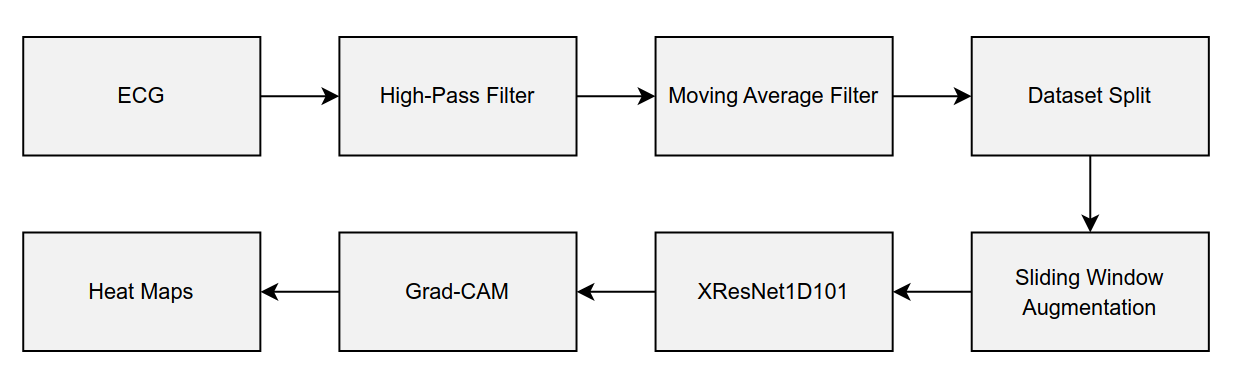
\includegraphics[width=\columnwidth]{flow.png}
    \caption{Overview of the proposed method}
    \label{fig:pipeline}
\end{figure}

\subsection{Multi-label Classification}
In the case of machine learning, many tasks primarily focus on classification, including binary and multiclass classification. However, a third classification paradigm, equally crucial yet often less discussed, is multi-label classification (MLC). In a multi-label scenario, each data sample can belong to more than one class instead of having one correct class. Formally, let the label space be
\[
\mathcal{Y} = \{y_1, y_2, \dots, y_L\},
\]
where $L$ is the total number of possible labels. For each sample $x \in \mathcal{X}$, the model outputs a vector of probabilities
\[
\hat{\mathbf{y}} = [\hat{y}_1, \hat{y}_2, \dots, \hat{y}_L], \quad \hat{y}_i \in [0,1],
\]
indicating the likelihood of the presence of each label $y_i$. Unlike single-label settings, the function must map each $\hat{y}_i$ into a binary value, yielding the final multi-label decision function:
\[
\mathbf{y}^\ast =
\big[ \mathbf{1}\{\hat{y}_1 \geq \tau_1\},
      \mathbf{1}\{\hat{y}_2 \geq \tau_2\},
      \dots,
      \mathbf{1}\{\hat{y}_L \geq \tau_L\} \big].
\]
where $\tau_i$ denotes the decision threshold for class $i$. In multi-label classification, a sample may belong to multiple classes simultaneously, which precludes selecting only the maximum probability as the final output. Since the number of positive labels is not predetermined, each class must be assessed independently. Accordingly, class-specific thresholds are required to convert predicted probabilities into binary decisions. For example, suppose a model outputs
\[
\hat{\mathbf{y}} = [0.058, 0.162, 0.665, 0.088, 0.767].
\]
With a uniform threshold of $\tau = 0.5$, the final decision becomes
\[
\mathbf{y}^\ast = [0, 0, 1, 0, 1].
\]
However, a single global threshold may not suit all classes, since each label may have different prevalence, importance, or discriminative difficulty. To address this, thresholds $\tau_i$ can be optimized independently for each class based on evaluation metrics such as the \textit{F1-score}, which balances precision and recall. Specifically, the optimal threshold for class $i$ is chosen as
\[
\tau_i^\ast = \arg\max_{\tau} \, F1_i(\tau),
\]
ensuring that class-wise predictions achieve the best trade-off between sensitivity and specificity. By adopting this approach, the model transforms raw probability vectors into robust multi-label predictions. MLC introduces additional complexities, as the model must not only identify the relevant labels but also capture the potential relationships and dependencies among the labels. Effective MLC approaches need to address challenges such as high-dimensional label spaces, imbalanced label distributions, and partial or missing label information, which are not readily addressed by conventional single-label classification techniques \cite{tarekegn2024deep}. Having multi-label annotations on data enables more comprehensive and accurate prediction of disease status, going beyond just single-disease diagnosis, which can help provide better early intervention and disease management for patients \cite{maxwell2017deep}. In this work, we address both multi-label and multiclass classification tasks.

\subsection{Model Architecture}
The model proposed in this work is based on a one-dimensional convolutional neural network (1D-CNN), which is dedicated to time series analysis. We use the XResNet1D101 model introduced in \cite{strodthoff2020deep}, which is a 1D version of the ResNet family that uses residual connections to prevent vanishing gradients in deep networks. Residual blocks facilitate the passage of gradients through shortcut paths, which enhance the stability of training and make the model learn better features. The implementation is built on XResNet, which extends standard ResNet by applying several architectural optimizations. The proposed method helps preserve more temporal resolution and reduce computational costs. The model receives filtered and normalized 12-lead ECG signals as input and processes them using 101 layers of residual blocks. Batch normalization and re-centering mechanisms are applied to enhance convergence and stability. The design allows the model to extract hierarchical spatial features from ECG signals while maintaining low computational overhead, making it suitable for real-time or embedded diagnostic applications.

\subsection{Explainability with Grad-CAM}
To address the black-box nature of deep learning models, in particular CNNs, and to increase trust in their predictions in application contexts such as medical diagnosis, explainability methods are essential. In this study, we employed Gradient-weighted Class Activation Mapping (Grad-CAM), an established explainability method introduced by Selvaraju et al.~\cite{selvaraju2017grad}, to provide visual insights into the model's predictions. Grad-CAM generates class-specific activation heatmaps that visually highlight the regions of the input signal most influential to the model's prediction. The underlying mechanism involves backpropagating the gradients of the predicted class score to the final convolutional layer of the neural network. These gradients are then used to weight the corresponding feature maps, followed by a Rectified Linear Unit (ReLU) activation to focus on features that positively influence the target class prediction. This process results in a coarse localization map that can be overlaid onto the original input, indicating where the model is ``looking'' to make its decision. One of the main benefits of Grad-CAM is that it can be applied to most CNN structures without adding extra architectural complexity; therefore, there is no need for re-training the model. In this work, Grad-CAM is combined with the XResNet1D101 model for classification. Using Grad-CAM, heatmaps are overlaid directly on the processed ECG data, revealing specific time segments and leads contributing most to the classification. The use of Grad-CAM in this study underscores its role as a powerful tool for advancing ECG analysis, fostering transparency, and contributing to the development of more reliable and clinically acceptable machine learning solutions for cardiovascular disease.
\FloatBarrier

%% ------------------------------------------------------------------
\section{Experimental Results}
\label{sec:results}
\subsection{PTB-XL}
The PTB-XL dataset, curated and released by Germany's Physikalisch-Technische Bundesanstalt (PTB), is an extensive collection of electrocardiogram data. This dataset contains more than 21,000 ECG recordings obtained from 18,885 patients, each featuring the standard 12 leads and spanning 10 seconds. It maintains a gender balance, with about 52\% of the subjects being male and 48\% female. The dataset offers signals at both 100 Hz and 500 Hz sampling rates, allowing detailed temporal analysis for medical purposes. PTB-XL is acknowledged as one of the largest publicly available ECG datasets. Besides the raw ECG signals, it includes comprehensive clinical metadata, such as patient age, gender, and diagnostic information, which enhances its value for machine learning research in the healthcare domain. The annotation system in PTB-XL follows the Standard Communication Protocol for ECG (SCP-ECG)~\cite{iso2009} and organizes diagnostic labels in a hierarchical structure. Labels fall into three non-exclusive categories: diag (e.g., anterior myocardial infarction), form (e.g., abnormal QRS morphology), and rhythm (e.g., atrial fibrillation). A total of 71 diagnostic statements are defined. Importantly, each ECG recording in PTB-XL can be annotated with multiple diagnostic labels simultaneously, making it a multi-label classification problem. For diagnostic statements, PTB-XL defines five major superclasses and 24 corresponding subclasses. The five superclasses are as follows:
\begin{itemize}
    \item \textbf{NORM}: Normal ECG signal
    \item \textbf{MI}: Myocardial infarction, typically due to reduced blood flow to the heart muscle
    \item \textbf{CD}: Conduction disturbances, including heart blocks and abnormal electrical impulse propagation
    \item \textbf{STTC}: ST/T-wave changes that may indicate cardiac pathology or physiological variations
    \item \textbf{HYP}: Hypertrophy, such as in hypertrophic cardiomyopathy (HCM), where the heart muscle is abnormally thickened
\end{itemize}

Overall, PTB-XL offers a valuable and varied asset that supports cutting-edge research in ECG-based disease identification and promotes the creation of more generalizable and interpretable machine learning solutions for cardiovascular medical care.

\begin{figure*}[!t]
    \centering
    \subfloat[Low-frequency noise (0.5 Hz) superimposed on the signal]{%
        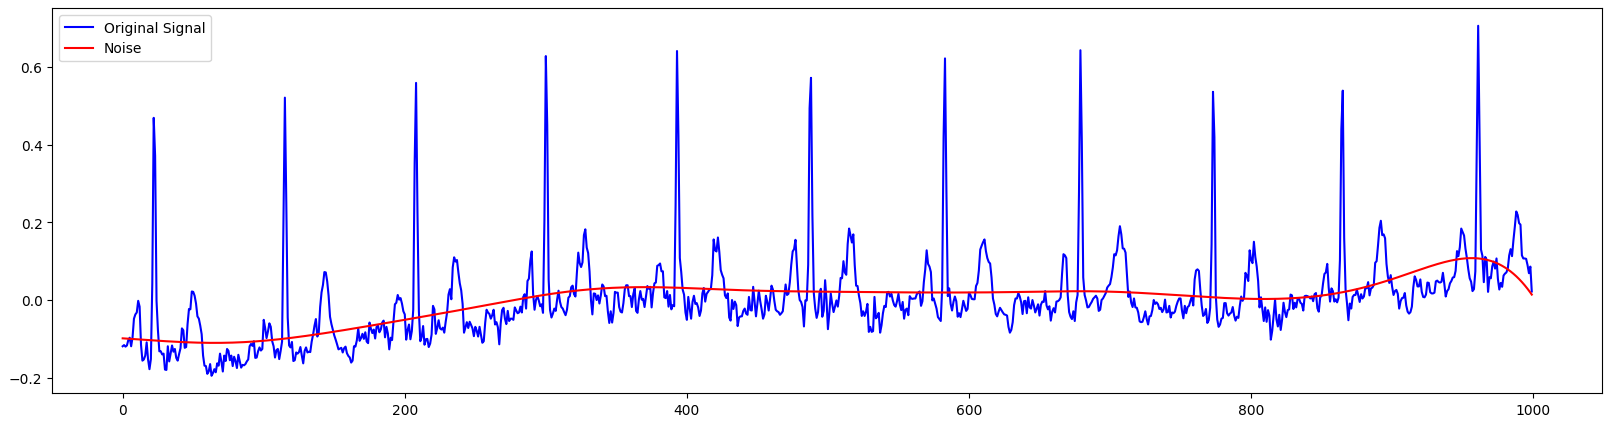
\includegraphics[width=0.48\textwidth]{baseline-a.png}%
    }
    \hfill
    \subfloat[Unwanted fluctuations]{%
        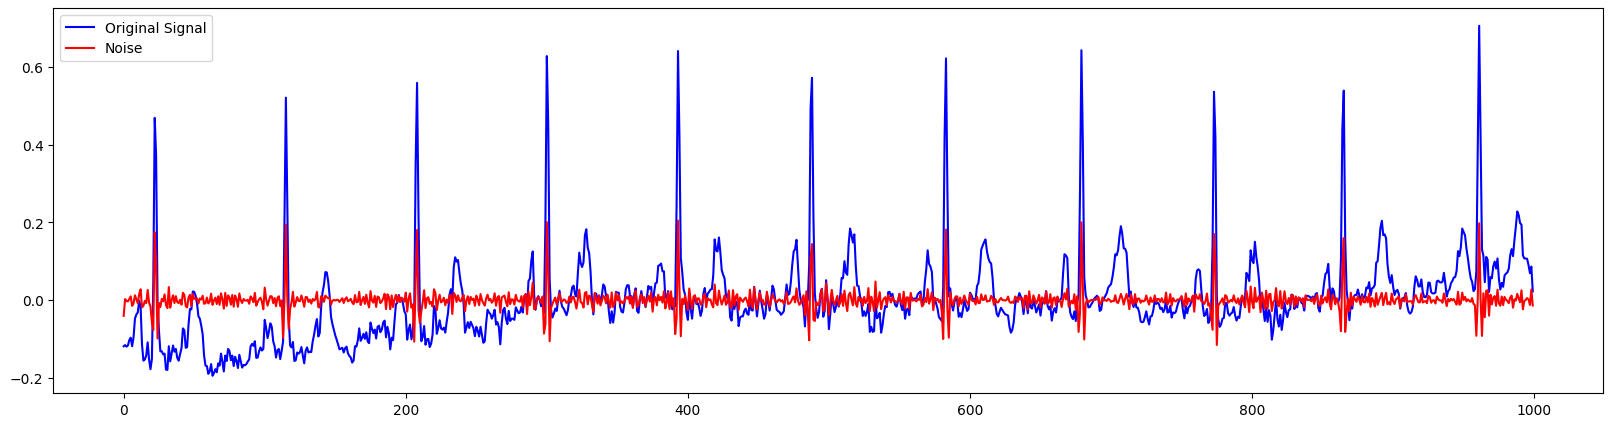
\includegraphics[width=0.48\textwidth]{variations-b.png}%
    }
    \caption{Typical noise distortions in ECG recordings.}
    \label{fig:ecg_noise_examples}
\end{figure*}

\subsection{Effects of Filtering}
ECG signals encompass typical types of noise. This makes them well-suited for assessing the effectiveness of preprocessing methods and algorithms that are resistant to noise. According to the National Center for Biotechnology Information (NCBI)~\cite{ncbi_ecg_basics}, the frequency range of a typical ECG is between 0.05 and 100 Hz, with the voltage amplitude in the range of 0.5 to 5 millivolts (mV). However, in the acquisition phase, the ECG is generally corrupted by external noise, and since the characteristics of the signal are key to diagnosis, the nature of the signal must remain the same. In our approach, we employed several FIR filter designs. The objective is to improve signal quality before classification while minimizing distortion of the original ECG morphology. First, a high-pass filter is applied to remove the baseline drift, with a cutoff frequency of 0.5 Hz. Then, to reduce high-frequency fluctuations and smooth the signal, a moving average filter is used, where each data point is replaced with the average of the surrounding data points (Fig.~\ref{fig:ecg_noise_examples}). The filter uses a window size of three, meaning that each output value is the average of the current value and the two surrounding values in the input signal. The effects of different filters are shown in Fig.~\ref{fig:noise2}.
\begin{figure}{}
\centering
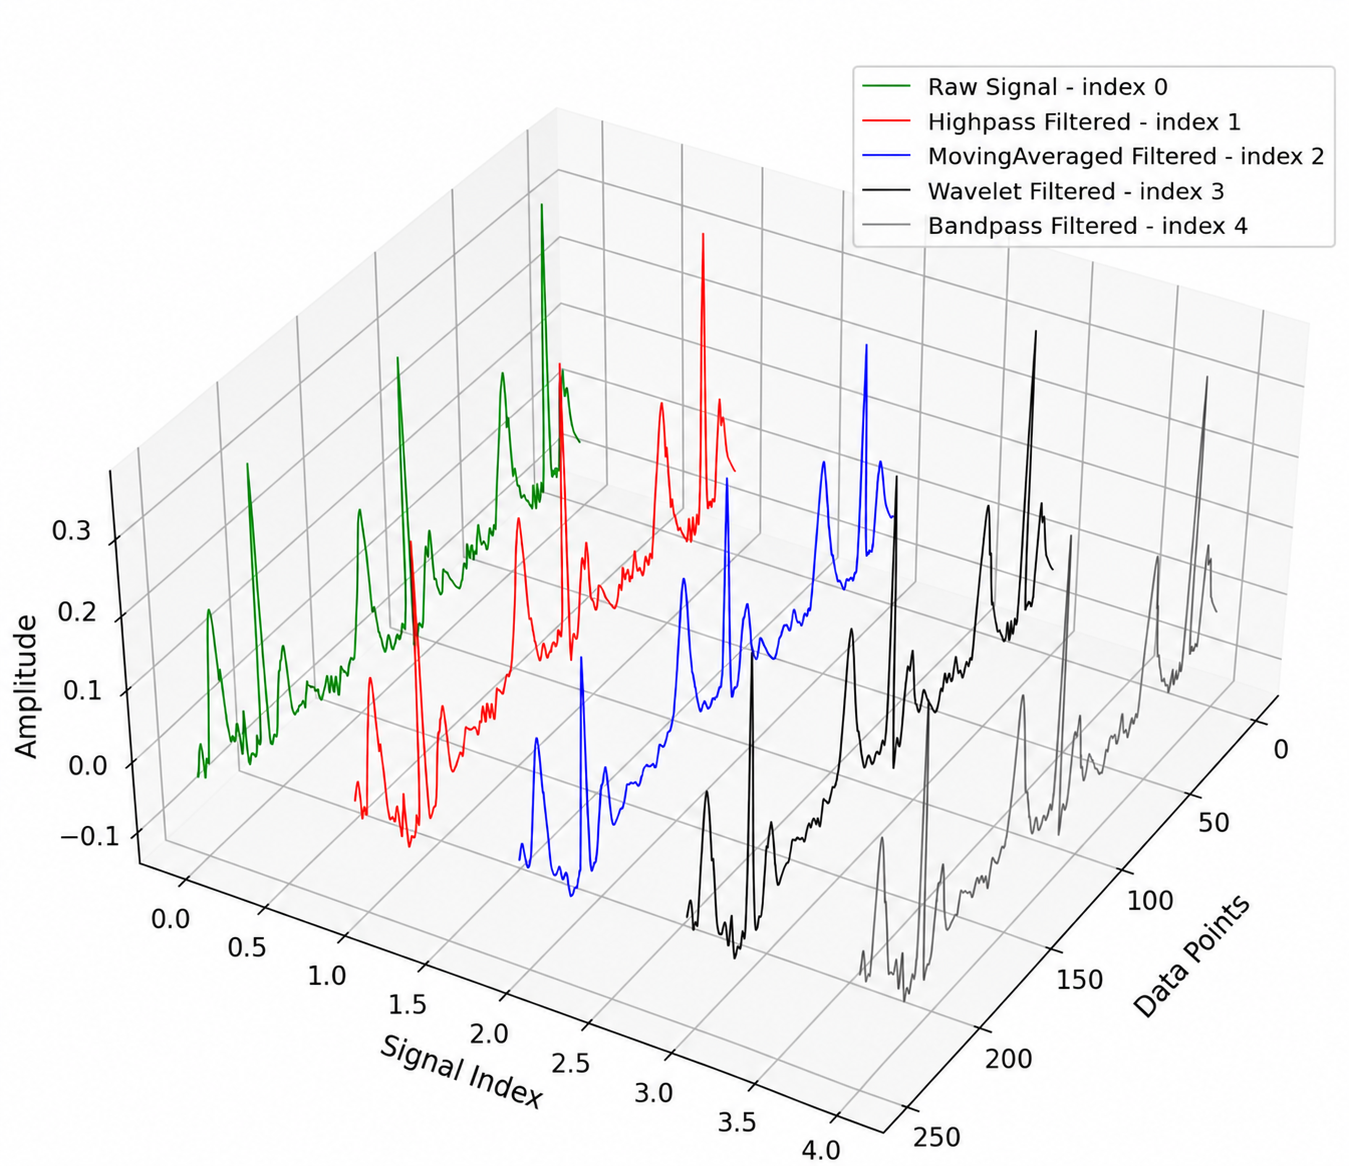
\includegraphics[width=0.85\columnwidth]{noise_fixed_amp.png}
\captionof{figure}{Impact of different denoising filters}
\label{fig:noise2}
\end{figure}
\subsection{Effects of Thresholds}
When determining the exact diagnosis for an electrocardiogram with a machine learning model, with validation from a cardiologist, the signal can be a symptom of multiple heart conditions, which the cardiologist might also suspect. A robust model must identify these possibilities and also consider the potential diagnoses. The PTB-XL dataset contains multi-label annotations, where the human validation for each patient's ECG signal can be assigned to multiple diagnoses, enabling it to belong to more than one category simultaneously. As a result, models and evaluation techniques must be capable of handling diverse outputs for each instance. To address this, we first trained a classifier on the entire training dataset, considering all aspects of the multi-label nature. In the second approach, we converted each cardiac condition --- Normal, Myocardial Infarction, ST/T Change, Conduction Disturbance, and Hypertrophy --- into a binary classification (presence or absence) and then evaluated the model's performance for each condition individually. When presented with a sample signal to diagnose the kind of cardiac condition, our model computes a probability associated with each potential heart condition. Determining the final diagnosis from this raw probability requires setting a threshold to decide whether the patient exhibits a particular condition. In other words, the probabilities calculated by the model are mapped into a binary output (0 or 1). In a multi-label scenario, where there may be more than one label, determining these thresholds becomes challenging. To address this, the optimal thresholds are calculated individually for each class by iteratively optimizing the F1-score. Then, these thresholds are implemented as the criterion for membership in a particular class. Fig.~\ref{fig:multi_fig} shows the effects of different thresholds on precision, recall, and F1-score. As shown, two points are marked on each curve. The red line indicates the threshold at which the F1-score reaches its maximum. The green line marks the intersection of the recall and precision curves, i.e., the threshold at which precision and recall are equal and therefore equal to the F1-score at that point. Since the F1-score balances both metrics, the red points are selected as the optimal thresholds for each class.

\begin{figure*}[!t]
  \centering
  \subfloat[CD\label{subfig:a}]{%
    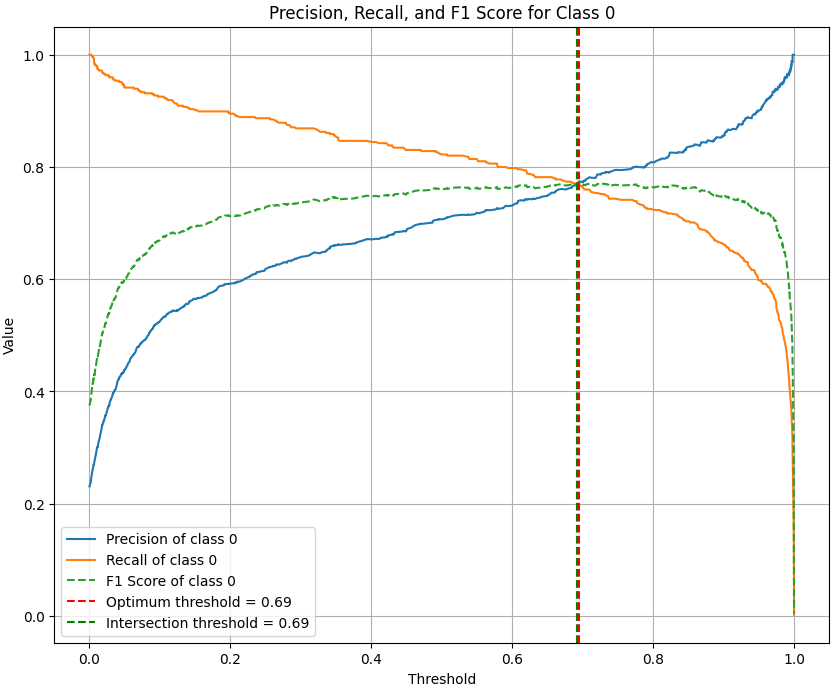
\includegraphics[width=0.32\textwidth]{thresh1.png}
  }
  \hfill
  \subfloat[HYP\label{subfig:b}]{%
    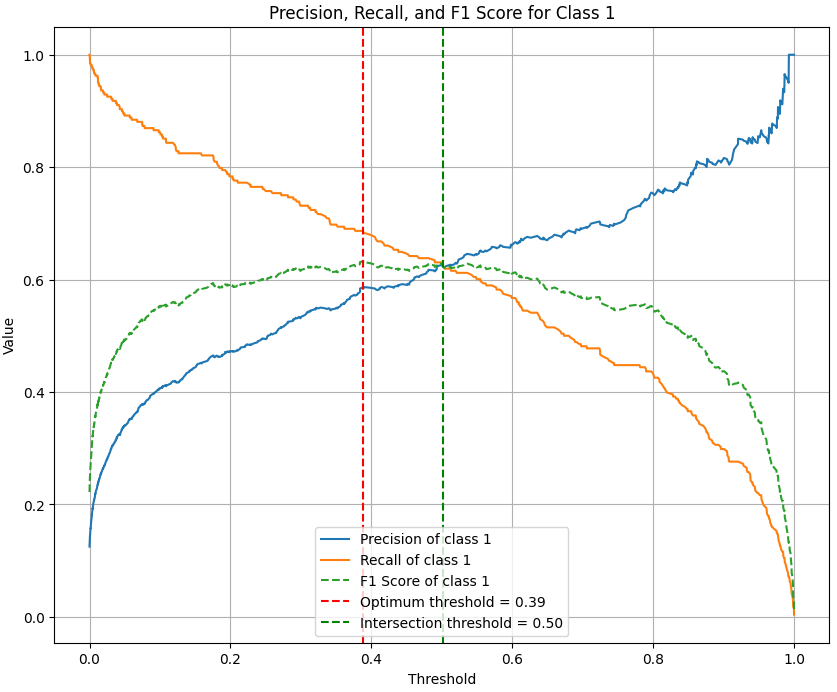
\includegraphics[width=0.32\textwidth]{thresh2.png}
  }
  \hfill
  \subfloat[MI\label{subfig:c}]{%
    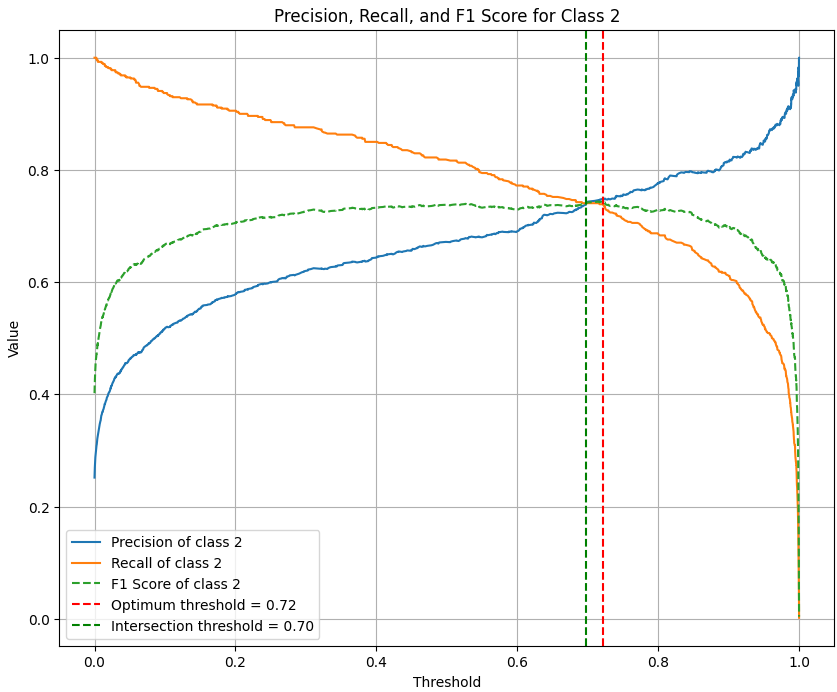
\includegraphics[width=0.32\textwidth]{thresh3.png}
  }
  \\
  \subfloat[NORM\label{subfig:d}]{%
    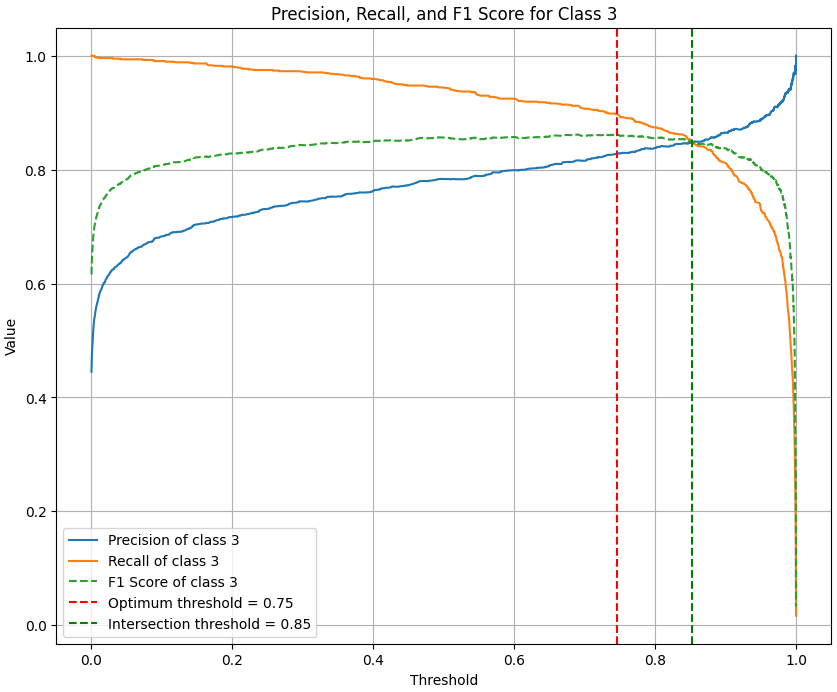
\includegraphics[width=0.32\textwidth]{thresh4.png}
  }
  \hspace{4mm}
  \subfloat[STTC\label{subfig:e}]{%
    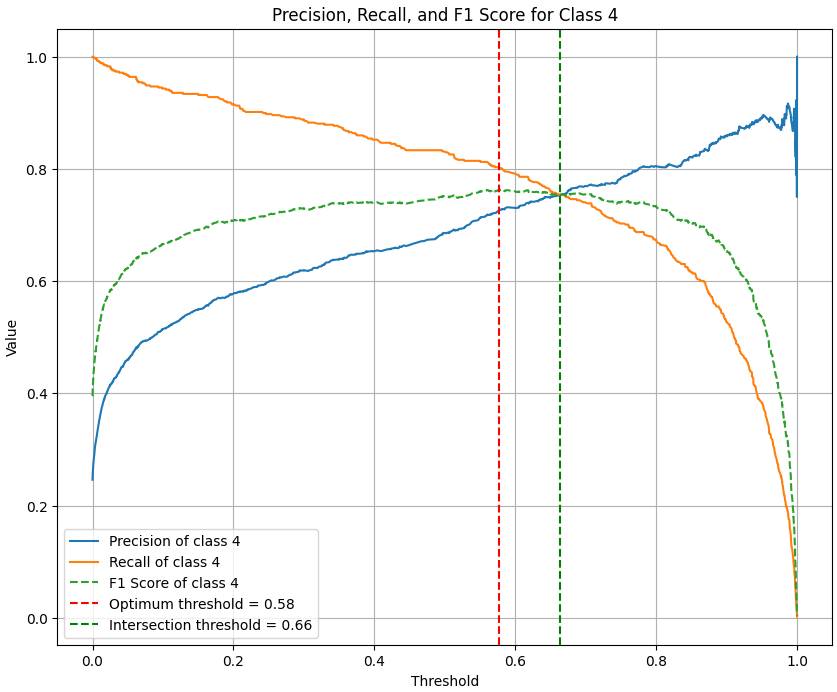
\includegraphics[width=0.32\textwidth]{thresh5.png}
  }
  \caption{Optimal threshold selection based on F1-score and final class determination}
  \label{fig:multi_fig}
\end{figure*}

\subsection{Training Setup and Evaluation Metrics}
\begin{figure}[]
\centering
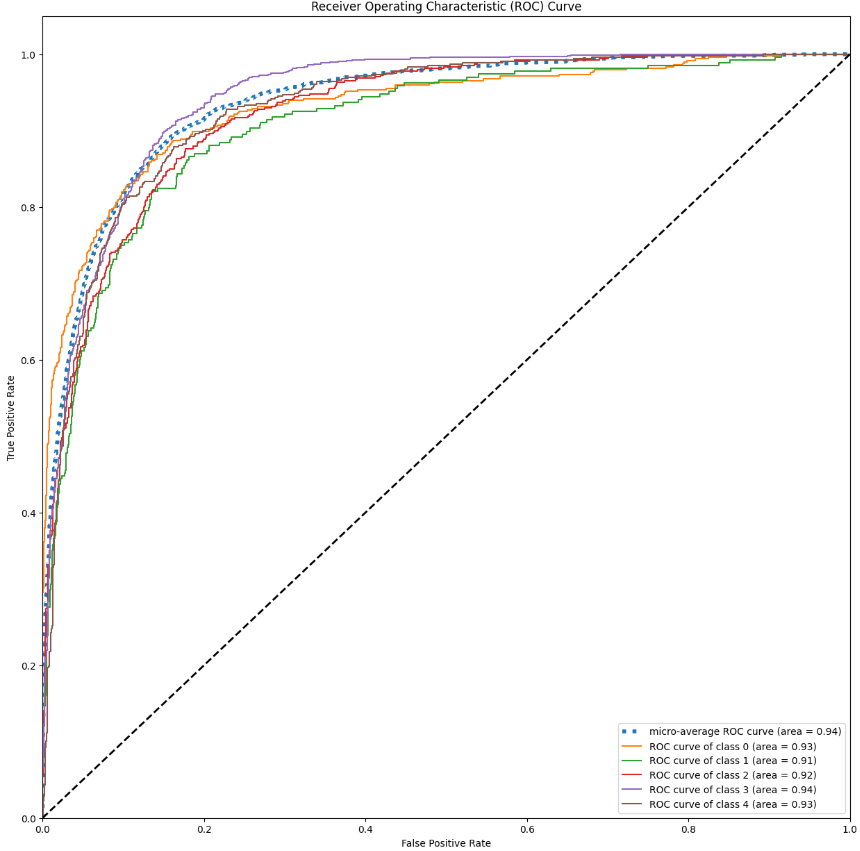
\includegraphics[width=\columnwidth]{ROC.png}
\caption{Receiver Operating Characteristic (ROC) curves with corresponding AUC values for each class, illustrating class-wise discriminative performance. The dotted curve is the micro-average (AUC = 0.94); the macro-average AUC is 0.93.}
\label{fig:roc}
\end{figure}
The model was trained on ECG signals, where high-pass filtering and moving average smoothing were applied as preprocessing steps. To mitigate overfitting, dropout was used, along with early stopping based on the macro-averaged AUC with a patience of seven epochs. Class-specific thresholds are used to map raw probabilities into binary outputs. In the multi-label setting, final classification decisions cannot be derived simply by selecting the maximum probability output. Instead, class-specific thresholds are required to map predicted probabilities into binary decisions. To ensure balanced performance, thresholds were optimized individually for each class using the \textit{F1-score}, which captures the trade-off between precision and recall. As a result, each cardiac condition was assigned its own optimal threshold, leading to more reliable predictions. The impact of this threshold tuning from Fig.~\ref{fig:multi_fig} is summarized in Table~\ref{tab:res}.

\begin{table}[!htb]
\centering
\caption{Evaluation results across classes}
\small
\begin{tabular}{|c|c|c|c|c|c|}
\hline
{\bfseries Class} & {\bfseries Accuracy} & {\bfseries Recall} & {\bfseries Precision} & {\bfseries F1-score} & {\bfseries AUC} \\
\hline
CD    & 0.89 & 0.73  & 0.79  & 0.758 & 0.93  \\
\hline
HYP   & 0.90 & 0.61  & 0.658 & 0.633 & 0.91  \\
\hline
MI    & 0.87 & 0.779 & 0.69  & 0.733 & 0.92  \\
\hline
NORM  & 0.87 & 0.926 & 0.805 & 0.86  & 0.94  \\
\hline
STTC  & 0.88 & 0.837 & 0.671 & 0.745 & 0.93  \\
\hline
Overall & 0.88 & 0.776 & 0.723 & 0.746 & 0.93  \\
\hline
\end{tabular}
\label{tab:res}
\end{table}
Overall, the model achieved strong classification performance with a micro-average AUC of 0.94. The use of optimized thresholds in a multi-label framework significantly improved prediction reliability, allowing the model to correctly identify multiple co-occurring cardiac conditions. Fig.~\ref{fig:roc} presents the corresponding ROC curves for each class, further illustrating the model's class-wise discriminative performance.
\subsection{Grad-CAM Heatmap Analysis}
To better understand how the proposed deep learning model makes its predictions, Grad-CAM was employed as an explainability technique. The purpose of this analysis is to reveal which regions of the electrocardiogram signals most strongly influenced the model's decisions. In this study, the focus of explainability is primarily on the \textbf{temporal occurrence of individual ECG waves}. When applying Grad-CAM, the raw heatmaps produced by the final convolutional layer have dimensions determined by the feature maps (e.g., $256 \times 32$). According to the original ECG signal length (e.g., $1000$), postprocessing was needed to align heatmaps with the input signal (Fig.~\ref{fig:normalleads}). It was observed that the horizontal axis (time) remains consistent across scales, preserving the alignment of cardiac events such as beats. However, the vertical axis (amplitude) values do not retain fixed positions and may shift depending on the rescaling. This introduces distortions that complicate the interpretation of morphological features. To overcome this limitation, an \textbf{averaging-based alignment strategy} is proposed. For each time step $t$, the values across all feature map channels are averaged:
\begin{equation}
\hat{H}(t) = \frac{1}{n} \sum_{i=1}^{n} H_i(t),
\end{equation}
Here, $H_i(t)$ denotes the heatmap value of feature map $i$ at time $t$, and $n$ is the total number of feature maps.
This operation produces a one-dimensional importance signal aligned with the ECG time axis. The visualizations highlight QRS complexes and P waves (Fig.~\ref{fig:reds}), while misclassified samples are examined morphologically. Fig.~\ref{fig:mileads} illustrates an example that was incorrectly classified as normal, even though it actually belongs to the MI class. Some leads, such as II, aVL, and V2, display irregular spacing between beats, which may have contributed to the model's mistake. The probabilities predicted by the model for this signal are: $[0.028784, 0.009288, 0.450851, 0.861472, 0.007335]$.
This indicates that the model focused on regions corresponding to MI signs in some areas, but not consistently across all parts, resulting in an overall probability of about 45\%. These visualizations are intended to enhance the interpretability and clinical trustworthiness of the system, bridging the gap between automated deep learning classification and human expert reasoning.
    \begin{figure}[!t]
    \centering
    \subfloat[I]{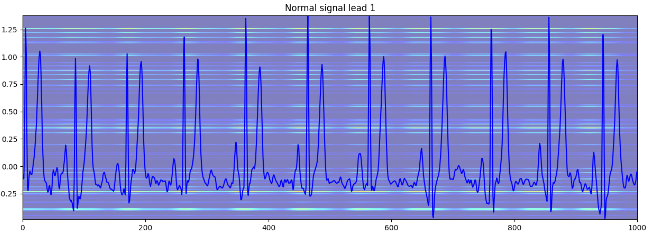
\includegraphics[width=0.48\columnwidth, height=2.2cm]{lead1.png}}\hfill
    \subfloat[II]{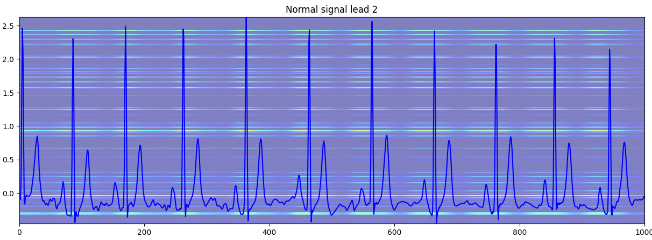
\includegraphics[width=0.48\columnwidth, height=2.2cm]{lead2.png}} \\
    \subfloat[III]{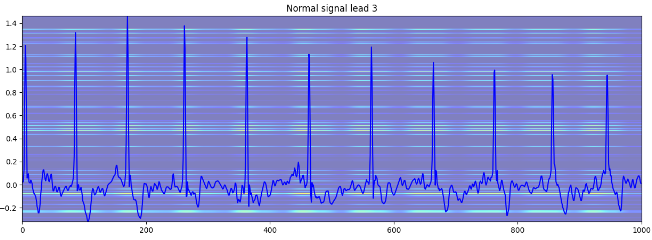
\includegraphics[width=0.48\columnwidth, height=2.2cm]{lead3.png}}\hfill
    \subfloat[aVR]{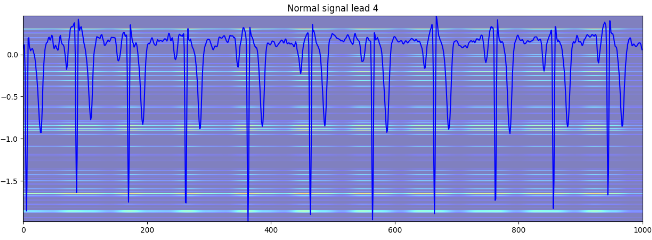
\includegraphics[width=0.48\columnwidth, height=2.2cm]{lead4.png}} \\
    \subfloat[aVL]{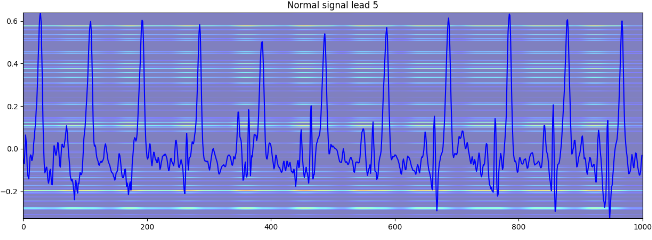
\includegraphics[width=0.48\columnwidth, height=2.2cm]{lead5.png}}\hfill
    \subfloat[aVF]{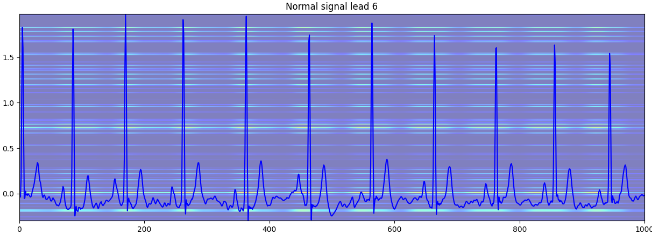
\includegraphics[width=0.48\columnwidth, height=2.2cm]{lead6.png}} \\
    \subfloat[V1]{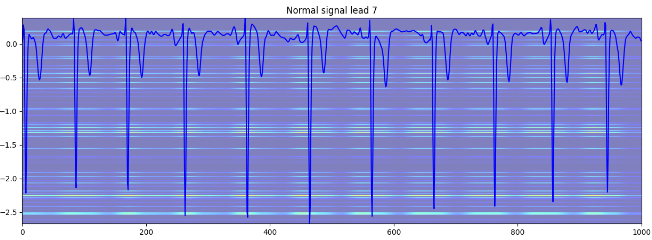
\includegraphics[width=0.48\columnwidth, height=2.2cm]{lead7.png}}\hfill
    \subfloat[V2]{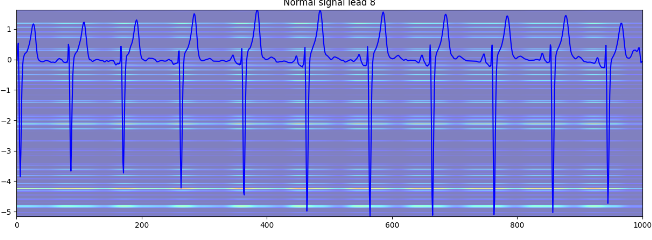
\includegraphics[width=0.48\columnwidth, height=2.2cm]{lead18.png}} \\
    \subfloat[V3]{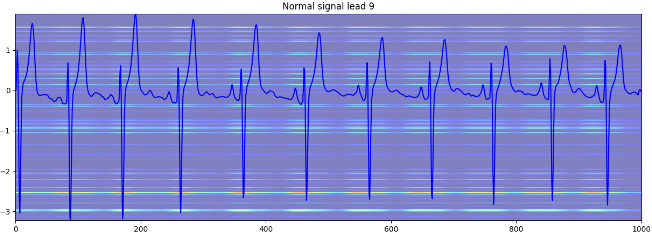
\includegraphics[width=0.48\columnwidth, height=2.2cm]{lead9.png}}\hfill
    \subfloat[V4]{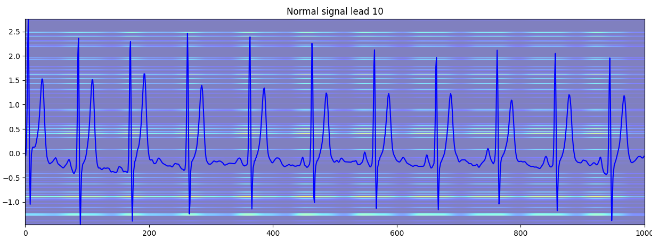
\includegraphics[width=0.48\columnwidth, height=2.2cm]{lead10.png}} \\
    \subfloat[V5]{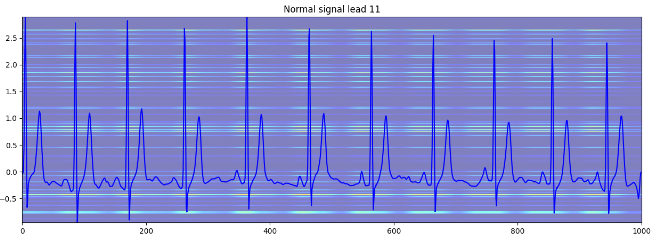
\includegraphics[width=0.48\columnwidth, height=2.2cm]{lead11.png}}\hfill
    \subfloat[V6]{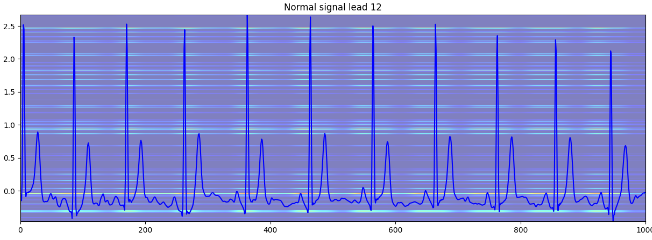
\includegraphics[width=0.48\columnwidth, height=2.2cm]{lead12.png}}
    \caption{Visualization of raw Grad-CAM heatmaps for the 12 leads (a--l) corresponding to a correct classification of the normal class. The blue waveform represents the filtered ECG signal. The horizontal background bands represent the individual feature map channels (32 channels) of the final convolutional layer; blue regions indicate low model activation, while brighter regions show where the model is extracting features to support its 'Normal' prediction. These raw heatmaps are later averaged to produce the one-dimensional importance signals shown in Fig.~\ref{fig:reds}.}
    \label{fig:normalleads}
\end{figure}
\newpage
\begin{figure*}[!t]
\centering
\subfloat[Lead I]{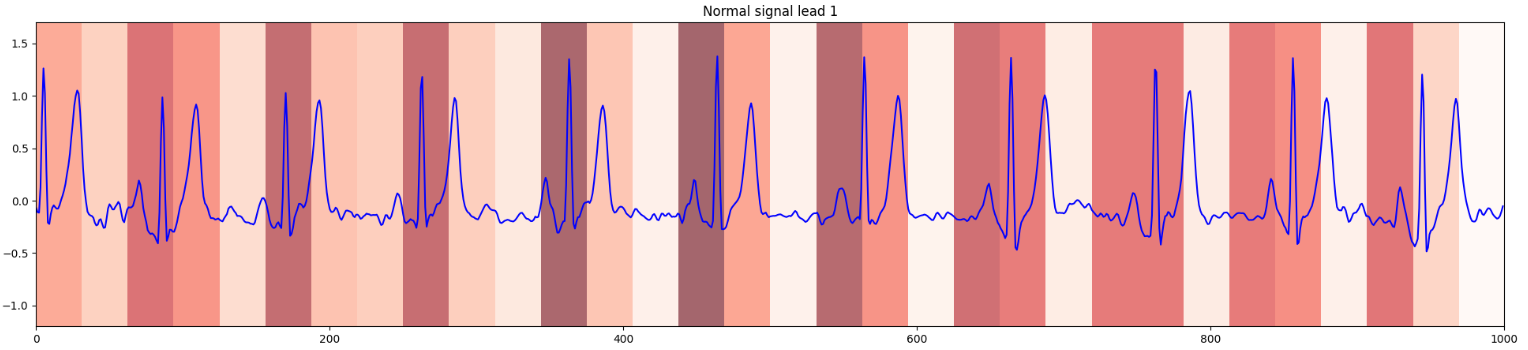
\includegraphics[width=0.48\textwidth]{reds1.png}}\hfill
\subfloat[Lead II]{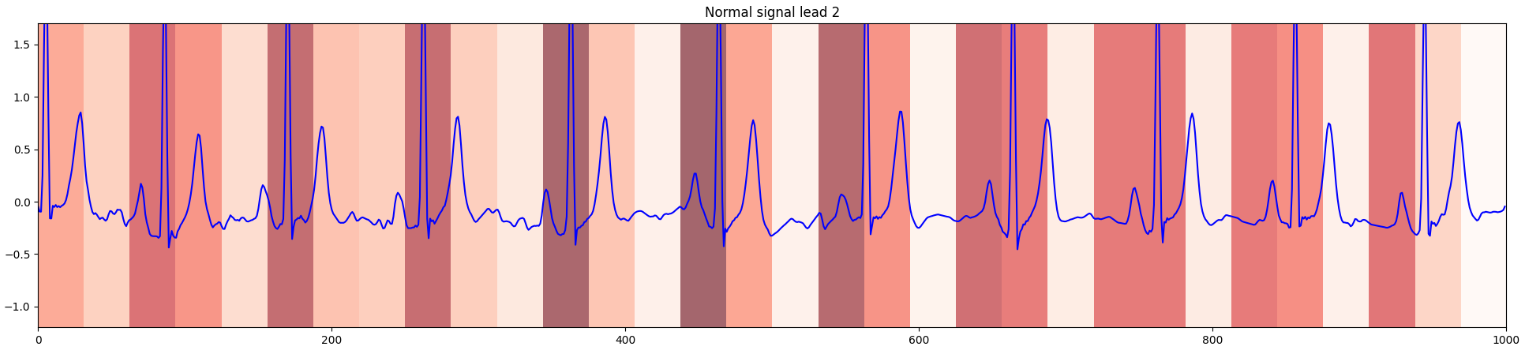
\includegraphics[width=0.48\textwidth]{reds2.png}} \\
\subfloat[Lead III]{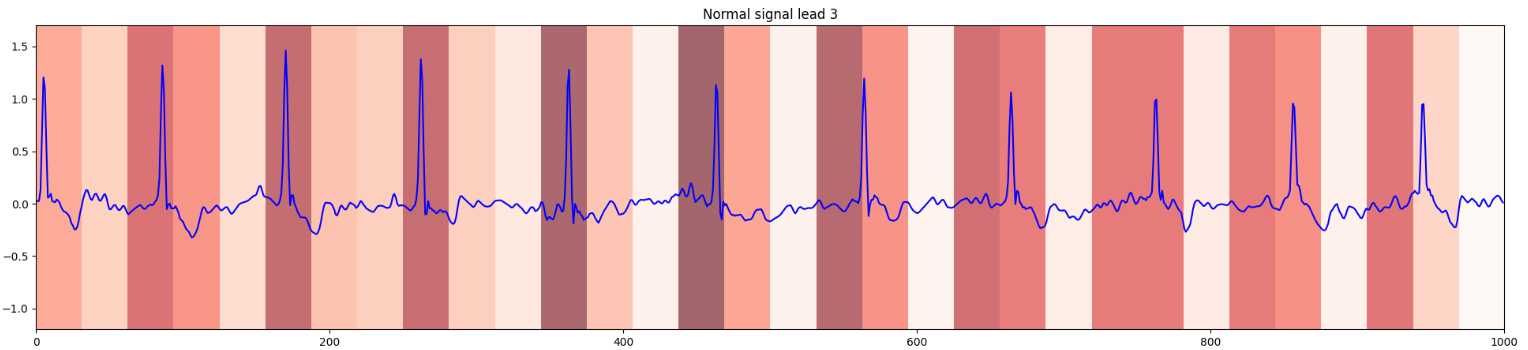
\includegraphics[width=0.48\textwidth]{reds3.png}}
\caption{Leads I to III visualized with heatmaps obtained through averaging, corresponding to the correct classification of the Normal class. (The horizontal axis represents time, and the vertical axis represents signal amplitude.)}
\label{fig:reds}
\end{figure*}

\begin{figure*}[!t]
    \centering
    \subfloat[I]{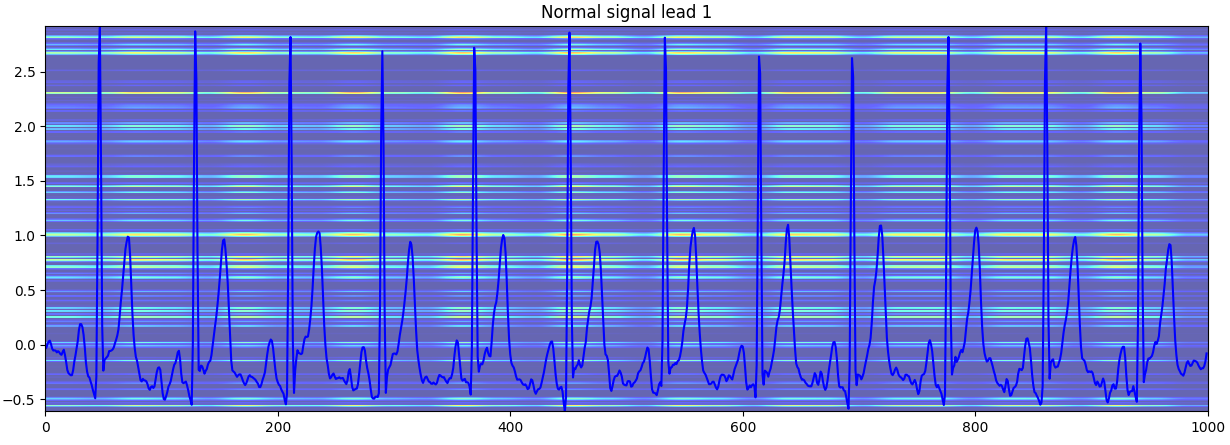
\includegraphics[width=0.32\textwidth, height=2.5cm]{milead2.png}}\hfill
    \subfloat[II]{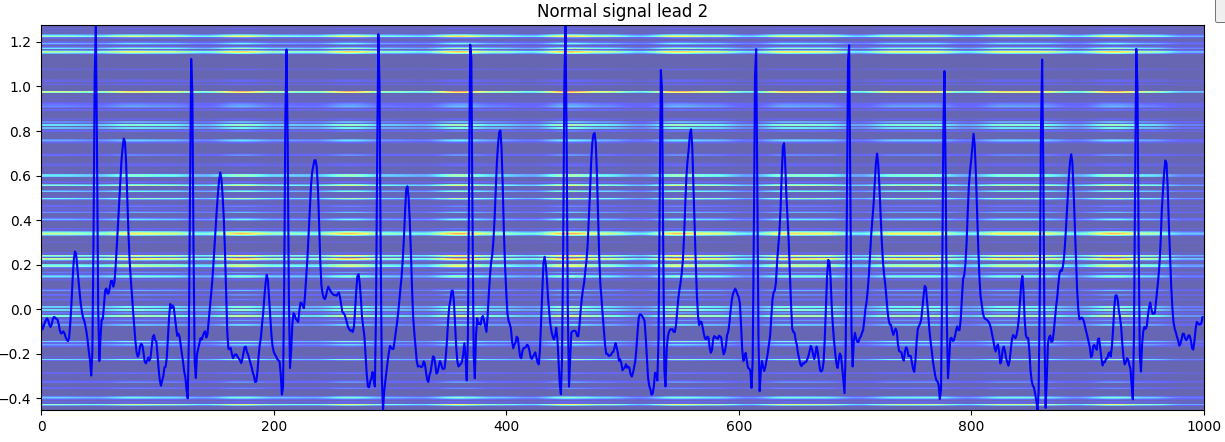
\includegraphics[width=0.32\textwidth, height=2.5cm]{milead3.png}}\hfill
    \subfloat[III]{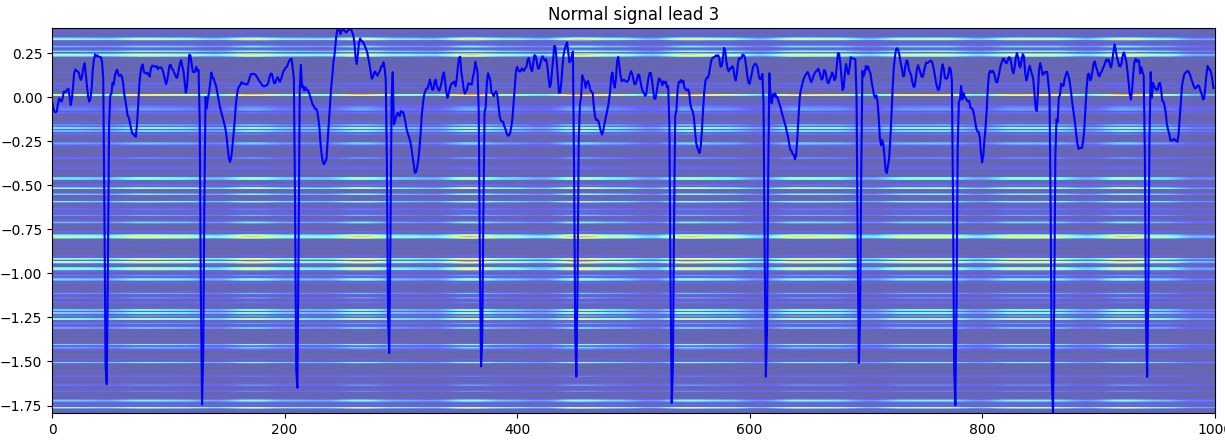
\includegraphics[width=0.32\textwidth, height=2.5cm]{milead4.png}} \\
    \subfloat[aVR]{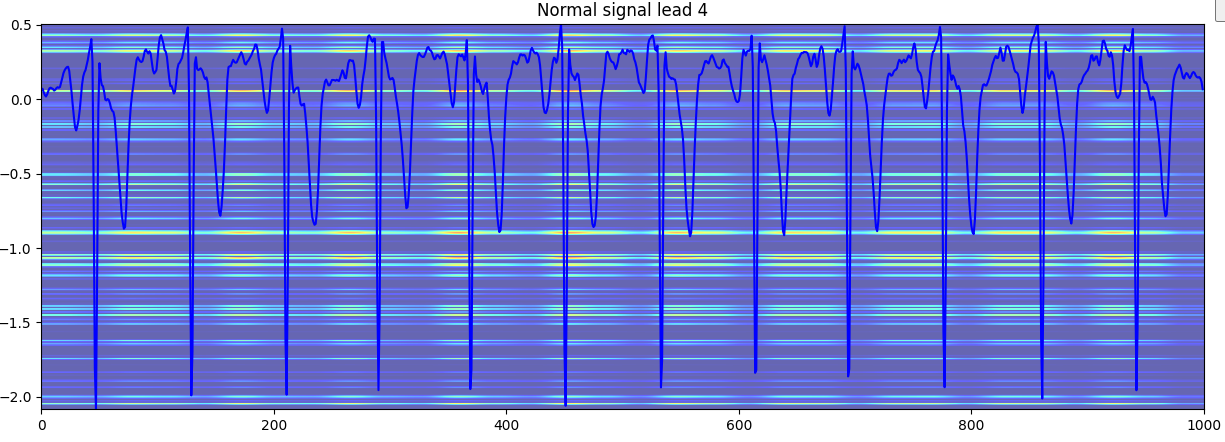
\includegraphics[width=0.32\textwidth, height=2.5cm]{milead5.png}}\hfill
    \subfloat[aVL]{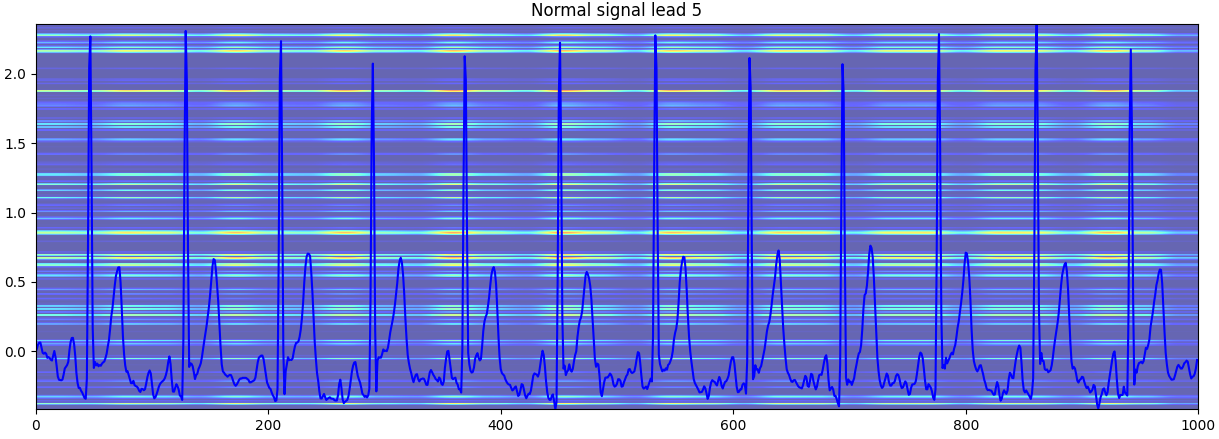
\includegraphics[width=0.32\textwidth, height=2.5cm]{milead6.png}}\hfill
    \subfloat[aVF]{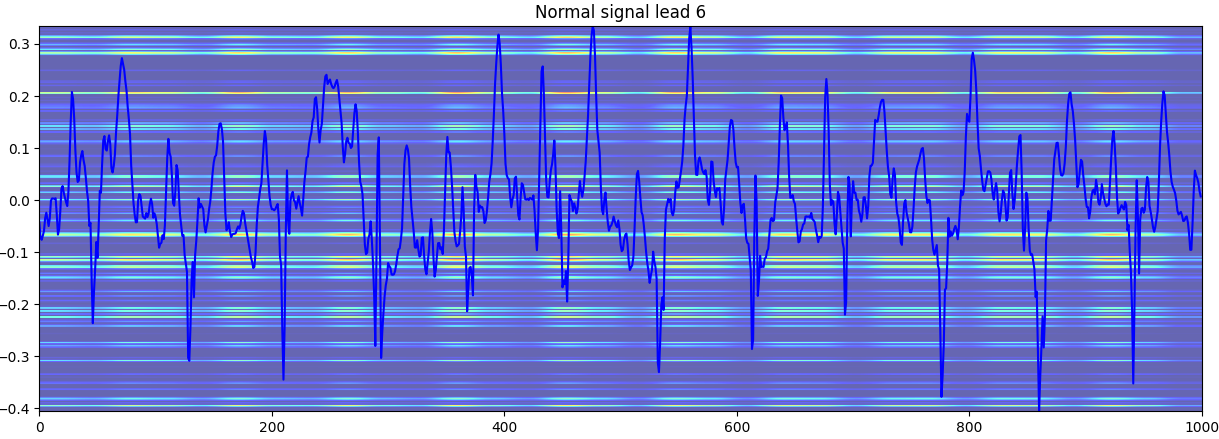
\includegraphics[width=0.32\textwidth, height=2.5cm]{milead7.png}} \\
    \subfloat[V1]{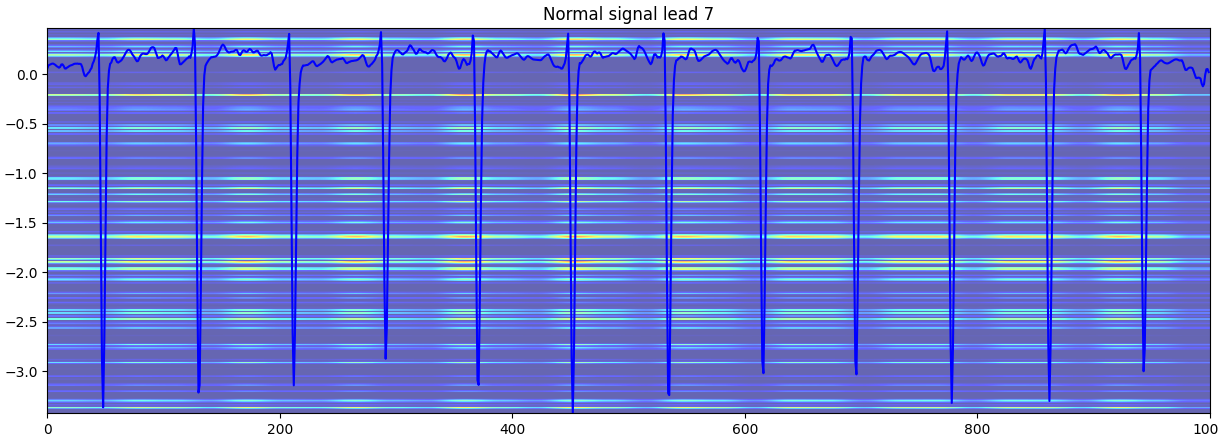
\includegraphics[width=0.32\textwidth, height=2.5cm]{milead8.png}}\hfill
    \subfloat[V2]{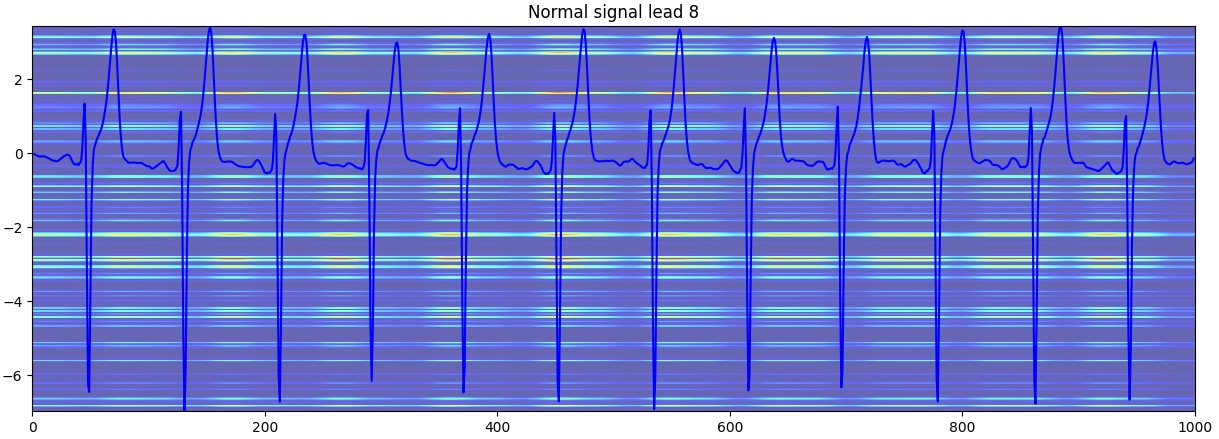
\includegraphics[width=0.32\textwidth, height=2.5cm]{milead9.png}}\hfill
    \subfloat[V3]{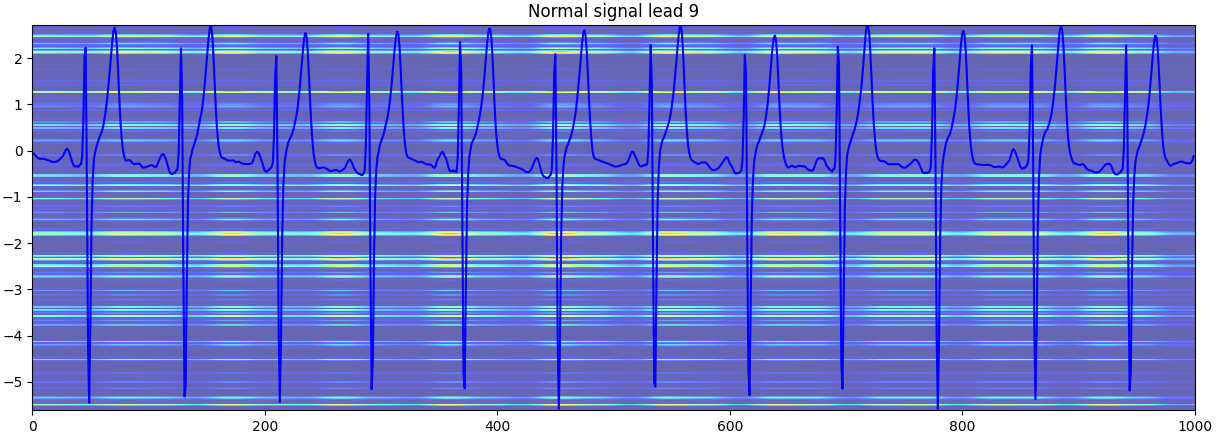
\includegraphics[width=0.32\textwidth, height=2.5cm]{milead10.png}} \\
    \subfloat[V4]{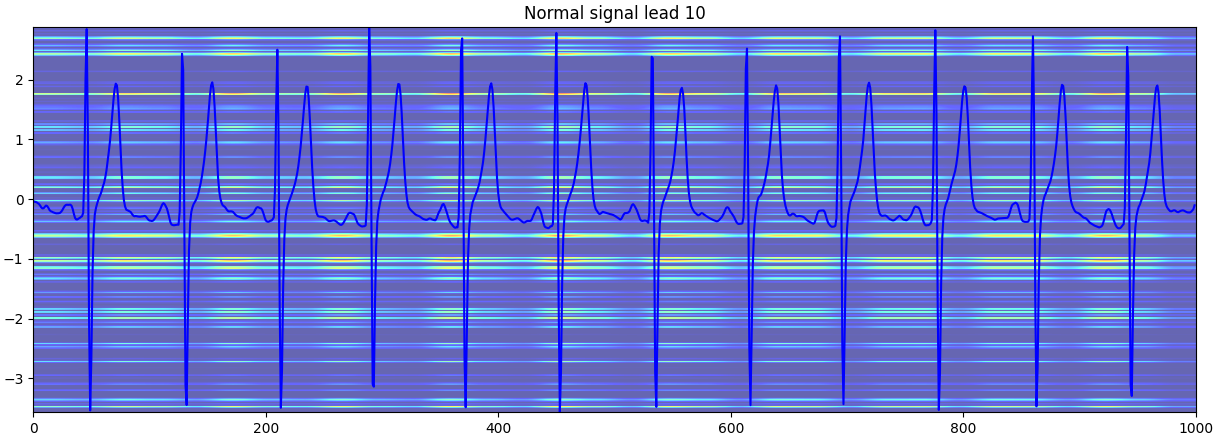
\includegraphics[width=0.32\textwidth, height=2.5cm]{milead11.png}}\hfill
    \subfloat[V5]{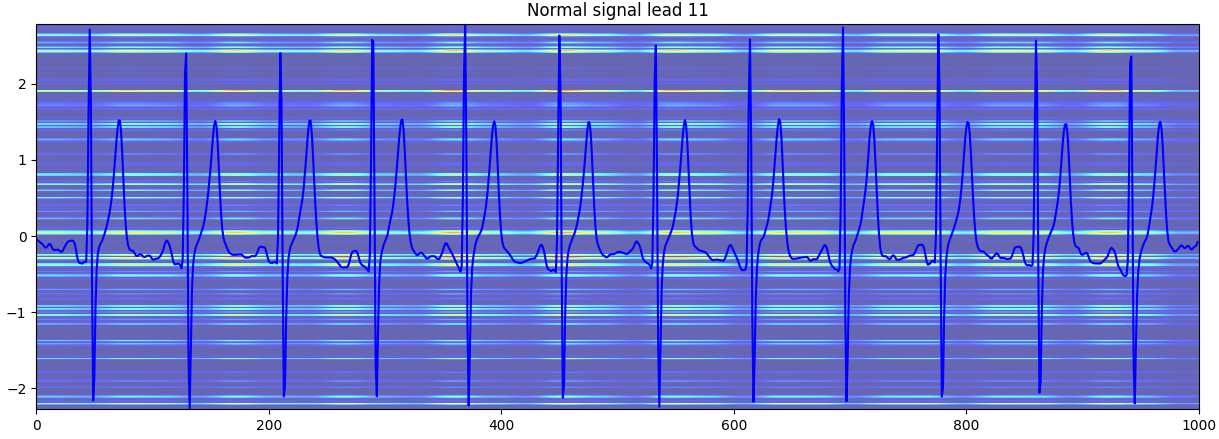
\includegraphics[width=0.32\textwidth, height=2.5cm]{milead12.png}}\hfill
    \subfloat[V6]{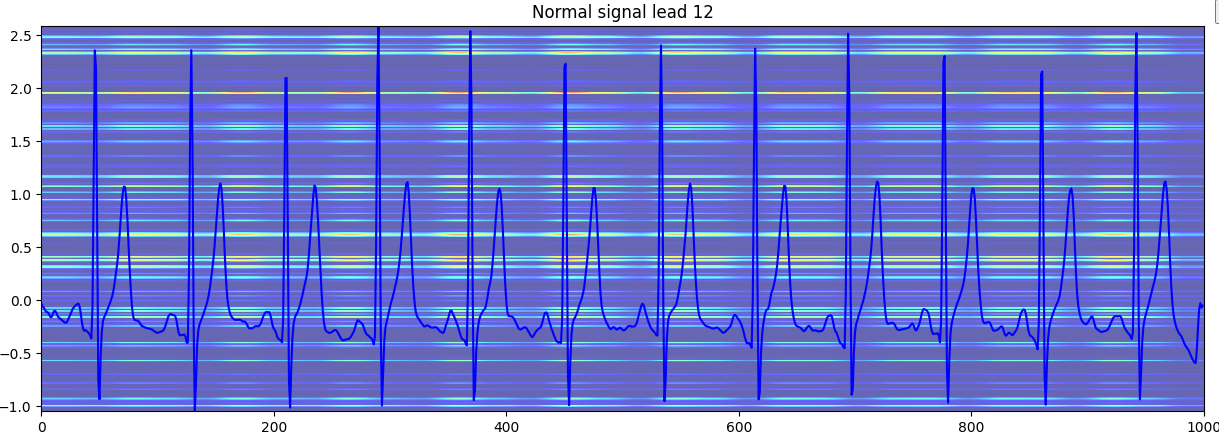
\includegraphics[width=0.32\textwidth, height=2.5cm]{milead13.png}}
    \caption{Misclassifications of the Normal class. (The horizontal axis represents time, and the vertical axis represents signal amplitude.)}
    \label{fig:mileads}
\end{figure*}
\FloatBarrier

%% ------------------------------------------------------------------
\section{Conclusion and Future Works}
\label{sec:conclusion}
In this study, we developed a multi-label deep learning approach for the classification of 12-lead ECG signals using an XResNet1D101 architecture. Instead of primarily focusing on single-label classification, this paper demonstrates the ability to simultaneously predict multiple cardiac conditions with an accuracy of around 88\%. This capability is of particular clinical importance, as several cardiac abnormalities may co-occur in practice. Additionally, using Grad-CAM on multi-label time series provides clinically interpretable visualizations that highlight signal regions contributing most to the model's predictions. This increases trust in automated diagnosis systems and enhances the potential applicability in medical decision-making. Positioning these results alongside recent studies helps clarify the contribution of the proposed method. Relative to lead-grouping architectures such as L5G-Net~\cite{yang2025lead}, our approach achieves comparable discriminative performance while additionally providing interpretability, suggesting that architectural strategies for modeling inter-lead relationships and explainability techniques may be complementary rather than competing directions for future work. Relative to heartbeat-level classifiers such as the attention-based model of Sundaramoorthy et al.~\cite{sundaramoorthy2026explainable}, the difference in reported accuracy is consistent with the differing granularity of the two tasks. What we highlight is a difference in the scope of interpretability: while attention-based mechanisms at the heartbeat level offer localized explanations, the Grad-CAM-based analysis presented here, supported by the proposed channel-averaging alignment strategy, extends interpretability across complete multi-lead recordings. This positions the proposed method as a complementary contribution within the broader landscape of explainable ECG classification. The evaluation was performed on the PTB-XL dataset, which, while comprehensive, presents challenges such as class imbalance and may not fully represent diverse real-world populations. Moreover, demographic, lifestyle, and genetic factors were not included in the analysis, which could provide a more holistic understanding of ECG-based diagnosis. Future work can address these limitations by incorporating additional and more diverse datasets, applying more advanced interpretability techniques, and exploring domain-specific data augmentation strategies (e.g., generative models) to mitigate class imbalance. Furthermore, integrating demographic and clinical metadata alongside ECG signals may improve both the robustness and the clinical relevance of the predictions. Overall, this research demonstrates that combining high-performing multi-label classification with model explainability offers a meaningful step toward clinically reliable machine learning solutions for cardiovascular disease diagnosis.

%% Elsevier-required statements (NOT in the IEEE version; uncomment/fill in at submission if needed):
%% %% ------------------------------------------------------------------
%% \section*{Data and code availability}
%% The PTB-XL dataset analysed in this study is publicly available at PhysioNet (\url{https://physionet.org/content/ptb-xl/}). %% Add your code repository link here.
%% \section*{Ethics statement}
%% This study used only the publicly available, de-identified PTB-XL dataset; no new data were collected from human participants.
%% \section*{Funding}
%% %% State funding sources, or: This research did not receive any specific grant from funding agencies in the public, commercial, or not-for-profit sectors.
%% \section*{Declaration of competing interest}
%% The authors declare that they have no known competing financial interests or personal relationships that could have appeared to influence the work reported in this paper.
%% \section*{Declaration of generative AI and AI-assisted technologies in the writing process}
%% %% Edit to match what was actually used, or delete if not applicable.
%% During the preparation of this work the authors used [TOOL/SERVICE] in order to [REASON]. After using this tool, the authors reviewed and edited the content as needed and take full responsibility for the content of the publication.
%% \section*{Acknowledgments}
%% %% Optional

\bibliographystyle{elsarticle-num}
\bibliography{ref}

\end{document}